\documentclass[a4paper, 11pt, oneside]{book} % A4 paper size, default 11pt font size and oneside for equal margins

\newcommand{\plogo}{\fbox{$\mathcal{PL}$}} % Generic dummy publisher logo

\usepackage[utf8]{inputenc} % Required for inputting international characters
\usepackage[T1]{fontenc} % Output font encoding for international characters
\usepackage{fouriernc} % Use the New Century Schoolbook font
\usepackage{graphicx}
\usepackage{amsthm}
\usepackage{verbatim}
\usepackage{hyperref}
\graphicspath{ {./images/} }

%----------------------------------------------------------------------------------------
%	TITLE PAGE
%----------------------------------------------------------------------------------------

\begin{document} 

\begin{titlepage} % Suppresses headers and footers on the title page

	\centering % Centre everything on the title page
	
	\scshape % Use small caps for all text on the title page
	
	\vspace*{\baselineskip} % White space at the top of the page
	
	%------------------------------------------------
	%	Title
	%------------------------------------------------
	
	\rule{\textwidth}{1.6pt}\vspace*{-\baselineskip}\vspace*{2pt} % Thick horizontal rule
	\rule{\textwidth}{0.4pt} % Thin horizontal rule
	
	\vspace{0.75\baselineskip} % Whitespace above the title
	
	{\LARGE Calculus\\ 2\\} % Title
	
	\vspace{0.75\baselineskip} % Whitespace below the title
	
	\rule{\textwidth}{0.4pt}\vspace*{-\baselineskip}\vspace{3.2pt} % Thin horizontal rule
	\rule{\textwidth}{1.6pt} % Thick horizontal rule
	
	\vspace{2\baselineskip} % Whitespace after the title block
	
	%------------------------------------------------
	%	Subtitle
	%------------------------------------------------
	
	Kinetic Energy % Subtitle or further description
	
	\vspace*{3\baselineskip} % Whitespace under the subtitle
	
	%------------------------------------------------
	%	Editor(s)
	%------------------------------------------------
	
	Created By
	
	\vspace{0.5\baselineskip} % Whitespace before the editors
	
	{\scshape\Large Ben Cordova \\ Colin hay \\ Harry Margalotti \\} % Editor list
	
	\vspace{1.0\baselineskip} % Whitespace below the editor list
	
	
	\textit{Ithaca College \\} % Editor affiliation
	
	\vfill % Whitespace between editor names and publisher logo
	
	2019 % Publication year
	

\end{titlepage}
%----------------------------------------------------------------------------------------
\pagebreak{}
\centering % Centre everything on the title page
{\LARGE Intro\\} % Title
\vspace{0.5\baselineskip} % Whitespace before the editors
In this paper, we will be exploring the real world applications of calculating linear and angular velocities in different scenarios. We will model, a record, a helicopter, and the earth throughout the paper, in our equations.
\vspace{1.0\baselineskip} % Whitespace before the editors

{\LARGE Why Can't We Apply the Kinetic Energy Formula Directly? \\} % Title
\vspace{0.5\baselineskip} % Whitespace before the editors
We cannot use the formula for kinetic energy to directly estimate our models. This is because the formula for kinetic energy is linear, yet our models deal with angular velocity. In each model, the record, the helicopter blade, and the Earth, we are measuring the kinetic energy of an object about its axis. This requires us to use the slice and add modeling approach for integrals. By calculating the mass and velocity of individual slices we are able to estimate the total kinetic energy of an object.

\vspace{1.0\baselineskip} % Whitespace before the editors

{\LARGE The Record \\} % Title
\vspace{0.5\baselineskip} % Whitespace before the editors
To calculate the kinetic energy of a record as it plays on a record player we must "slice" the model into smaller parts. We have decided to think of the record as a collection of circular strips, radiating out from the center. This is convenient because our formula for angular velocity requires the object to be circular. By finding the angular velocity and mass of our slices, we are able to estimate the kinetic energy of the entire object. 

\vspace{0.5\baselineskip} % Whitespace before the editors
{\LARGE Get Mass of Slice \\} % Title
\vspace{0.5\baselineskip} % Whitespace before the editors
\textit{Kinetic Energy} = $\frac{1}{2}$(\textit{mass})(\textit{linear velocity})$^2$
\vspace{0.5\baselineskip} % Whitespace before the editors

To start we will think of the area of the record using the following model. By using the circumference of a circle, and thinking of our circular slice as a rectangle, we are able to effectively determine the mass of the record.

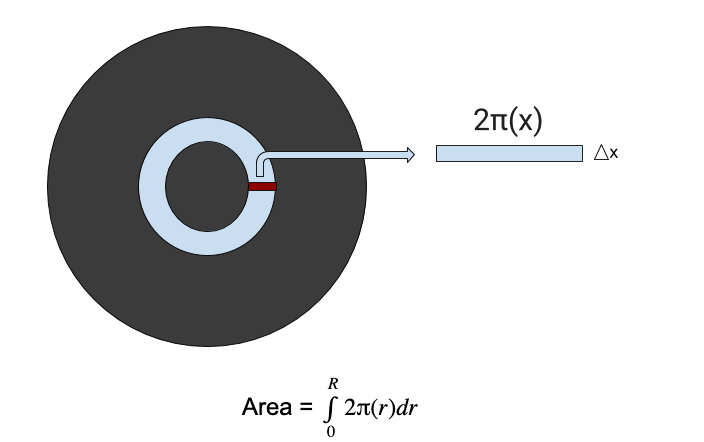
\includegraphics[scale=0.38]{record1}\\
Our first step is to get the mass of an individual slice. We do this by breaking down the formula for mass into smaller parts that we can directly relate to our record. Below is the formula for mass.\\
\vspace{0.5\baselineskip} % Whitespace before the editors
\vspace{0.5\baselineskip} % Whitespace before the editors
\textit{mass} = \textit{volume} $*$ \textit{density} \\
\vspace{0.5\baselineskip} % Whitespace before the editors
\vspace{0.5\baselineskip} % Whitespace before the editors
We then relate this formula to our record.\\
\vspace{0.5\baselineskip} % Whitespace before the editors
\vspace{0.5\baselineskip} % Whitespace before the editors
\textit{slice mass} = \textit{slice volume} $*$ \textit{record density}\\
\vspace{0.5\baselineskip} % Whitespace before the editors
\vspace{0.5\baselineskip} % Whitespace before the editors
Slice volume can be simplified further\dots below is a formula for volume.\\
\vspace{0.5\baselineskip} % Whitespace before the editors
\vspace{0.5\baselineskip} % Whitespace before the editors
\textit{volume} = \textit{area} $*$ \textit{thickness} \\
\vspace{0.5\baselineskip} % Whitespace before the editors
\vspace{0.5\baselineskip} % Whitespace before the editors
We then relate this formula to our record.\\
\vspace{0.5\baselineskip} % Whitespace before the editors
\vspace{0.5\baselineskip} % Whitespace before the editors
\textit{slice volume} = \textit{slice area} $*$ \textit{record thickness}\\
\vspace{0.5\baselineskip} % Whitespace before the editors
\vspace{0.5\baselineskip} % Whitespace before the editors
Slice area can be simplified further\dots below is a formula for area.\\
\vspace{0.5\baselineskip} % Whitespace before the editors
\vspace{0.5\baselineskip} % Whitespace before the editors
\textit{area} = \textit{length} $*$ \textit{width}\\
\vspace{0.5\baselineskip} % Whitespace before the editors
\vspace{0.5\baselineskip} % Whitespace before the editors
We then relate this formula to our record.\\
\vspace{0.5\baselineskip} % Whitespace before the editors
\vspace{0.5\baselineskip} % Whitespace before the editors
\textit{slice area = slice length $*$ $\Delta$ radius}
\vspace{0.5\baselineskip} % Whitespace before the editors
\vspace{0.5\baselineskip} % Whitespace before the editors
Slice length can be simplified further\dots we are now able to use our original model that sliced the area of a circle into radiating strips. Our model defined the length of one strip to be 
\vspace{0.5\baselineskip} % Whitespace before the editors
\vspace{0.5\baselineskip} % Whitespace before the editors
$2\pi r \blacksquare$ \\
\vspace{0.5\baselineskip} % Whitespace before the editors
\vspace{0.5\baselineskip} % Whitespace before the editors

\textit{slice length = $2\pi r$}

\vspace{0.5\baselineskip} % Whitespace before the editors
\vspace{0.5\baselineskip} % Whitespace before the editors
We have now simplified the formula for mass and related it directly to our record.\\
\vspace{0.5\baselineskip} % Whitespace before the editors
\vspace{0.5\baselineskip} % Whitespace before the editors
\textit{slice mass = $2\pi r * \Delta$radius $*$ record thickness $*$ record density}
\vspace{0.5\baselineskip} % Whitespace before the editors
\vspace{0.5\baselineskip} % Whitespace before the editors

{\LARGE Get Linear Velocity of Slice \\} % Title
\vspace{0.5\baselineskip} % Whitespace before the editors
\vspace{0.5\baselineskip} % Whitespace before the editors
Our next step is to get the linear velocity of an individual slice. Again we will break down the formula for linear velocity as it relates to angular velocity.\\

\vspace{0.5\baselineskip} % Whitespace before the editors
\vspace{0.5\baselineskip} % Whitespace before the editors
\textit{linear velocity = angular velocity $*$ radius}
\vspace{0.5\baselineskip} % Whitespace before the editors
\vspace{0.5\baselineskip} % Whitespace before the editors

We then relate this to our record.\\
\vspace{0.5\baselineskip} % Whitespace before the editors
\vspace{0.5\baselineskip} % Whitespace before the editors
\textit{slice linear velocity = record angular velocity $*$ radius}
\vspace{0.5\baselineskip} % Whitespace before the editors
\vspace{0.5\baselineskip} % Whitespace before the editors

We have now simplified formulas for mass and linear velocity as they relate to our record. We can now plug these into our formula for kinetic energy and use an integral to consider each slice. \\
\vspace{0.5\baselineskip} % Whitespace before the editors
\vspace{0.5\baselineskip} % Whitespace before the editors
\textit{kinetic energy = $\frac{1}{2} \int_{0}^{R}$slice mass $*$ slice linear velocity$^2$ dr}\\
\vspace{0.5\baselineskip} % Whitespace before the editors
\vspace{0.5\baselineskip} % Whitespace before the editors
We will now plug our simplifications for slice mass and slice linear velocity into this integral. \\
\vspace{0.5\baselineskip} % Whitespace before the editors
\vspace{0.5\baselineskip} % Whitespace before the editors
\textit{kinetic energy = $\frac{1}{2} \int_{0}^{R}(2\pi r * $record thickness $*$ record density) $*$ (record angular velocity $* r)^2 dr$}\\
\vspace{0.5\baselineskip} % Whitespace before the editors
\vspace{0.5\baselineskip} % Whitespace before the editors
This formula now shows us what characteristics of a record we should research to estimate the kinetic energy. We need to find values for radius, record thickness, record density, and record angular velocity. Below is a table with the values we found.\\
\begin{table}[!h]
\centering
\begin{tabular}{|l|l|l|l|}
\hline
Radius  & Thickness & Density                        & Angular Velocity \\
0.1524m & 0.001m    & $\frac{1350kg}{m^3}$    & $\frac{3.49065 rad}{s}$    \\
(6 in)  & (1mm)     & $(\frac{1.35 g}{cm^3})$ & $(33 \frac{1}{3} rpm)$\\
\end{tabular}
\end{table}
\vspace{0.5\baselineskip} % Whitespace before the editors
\vspace{0.5\baselineskip} % Whitespace before the editors
During our research we decided to focus on a 12 inch LP Record. We have found an estimate for the thickness (height) of a record from a forum post (see reference 1).\\
\vspace{0.5\baselineskip} % Whitespace before the editors
\vspace{0.5\baselineskip} % Whitespace before the editors
\textit{"many of the thinnest [LP Records] (0.9 to 1.0 mm) were the most uniform in thickness and some of the best sounding"}\\
\centering{\textit{-tketcham}}\\
\vspace{0.5\baselineskip} % Whitespace before the editors
\vspace{0.5\baselineskip} % Whitespace before the editors
\textit{$1mm * \frac{1m}{1000mm} = 0.001m$}\\
\vspace{0.5\baselineskip} % Whitespace before the editors
\vspace{0.5\baselineskip} % Whitespace before the editors

We then found from this source (see reference 4) that LP Records were commonly made out of polyvinyl chloride which typically has a density of 1.35 $\frac{g}cm^3$. Again we convert this to $\frac{kg}m^3$ to match the units of kinetic energy. \\
\vspace{0.5\baselineskip} % Whitespace before the editors
\vspace{0.5\baselineskip} % Whitespace before the editors
$(1.35\frac{g}{cm^3}) * (1\frac{kg}{1000g})*(1000000\frac{cm^3}{1m^3}) = 1350\frac{kg}{m^3}$\\
\vspace{0.5\baselineskip} % Whitespace before the editors
\vspace{0.5\baselineskip} % Whitespace before the editors
Finally we found from the LP Record wikipedia page (reference 2) that 12 inch records typically spun at 33 $\frac{1}{3}$ rpms. We then converted this to radians per second to match the units of kinetic energy.\\
\vspace{0.5\baselineskip} % Whitespace before the editors
\vspace{0.5\baselineskip} % Whitespace before the editors
$(33.3333 \frac{rev}{min})*(\frac{1min}{60s})*(\frac{2\pi rad}{1rev}) = 3.49065 \frac{rad}{s}$
\vspace{0.5\baselineskip} % Whitespace before the editors
\vspace{0.5\baselineskip} % Whitespace before the editors

{\LARGE Check Units \\} % Title
\vspace{0.5\baselineskip} % Whitespace before the editors
\vspace{0.5\baselineskip} % Whitespace before the editors

To confirm our previous work we are going to check the units of our formula given these values. Kinetic energy is typically measured in Joules: \\
\vspace{0.5\baselineskip} % Whitespace before the editors
\vspace{0.5\baselineskip} % Whitespace before the editors
$J=\frac{1kg*m^2}{s^2}$\\
\vspace{0.5\baselineskip} % Whitespace before the editors
\vspace{0.5\baselineskip} % Whitespace before the editors
The units for our formula are:\\
\vspace{0.5\baselineskip} % Whitespace before the editors
\vspace{0.5\baselineskip} % Whitespace before the editors
$m*m*(\frac{kg}{m^3})*(\frac{rad}{s} * m)^2*m$\\
\vspace{0.5\baselineskip} % Whitespace before the editors
\vspace{0.5\baselineskip} % Whitespace before the editors
$kg*\frac{m^2}{s^2}$\\ 
\vspace{0.5\baselineskip} % Whitespace before the editors
\vspace{0.5\baselineskip} % Whitespace before the editors

{\LARGE Estimate Kinetic Energy \\} % Title
\vspace{0.5\baselineskip} % Whitespace before the editors
\vspace{0.5\baselineskip} % Whitespace before the editors

As you can see the units for our formula model the units for Jules. This gives us confidence that the formula we derived for kinetic energy is accurate. Now we can plug assumed values into our formula to start estimating the kinetic energy of a record.\\

\vspace{0.5\baselineskip} % Whitespace before the editors
\vspace{0.5\baselineskip} % Whitespace before the editors

\textit{kinetic energy = $\frac{1}{2}\int_{0}^{0.1524}(2\pi r * 0.001*1350) * (3.49065 * r)^2 dr$}\\

\vspace{0.5\baselineskip} % Whitespace before the editors
\vspace{0.5\baselineskip} % Whitespace before the editors

\textit{kinetic energy = 0.00696909 Jules }\\

\vspace{0.5\baselineskip} % Whitespace before the editors
\vspace{0.5\baselineskip} % Whitespace before the editors

Our estimation for the kinetic energy of a 12 inch LP Record is 0.00696909 Jules. This estimate
has many flaws. One such flaw is that we are unsure if LP Records are made completely out of polyvinyl chloride. This impacts the density of the record and would change our result. We also did not account for the fact that a record would not have a constant density because of the grooves. We still have faith in our formula because the units correctly work out to give us the units for Joules, however our assumptions most likely introduced a significant amount of error. \\

\vspace{0.5\baselineskip} % Whitespace before the editors
\vspace{0.5\baselineskip} % Whitespace before the editors
---------------------------------------------------------------------------------------------------------
\vspace{0.5\baselineskip} % Whitespace before the editors
\vspace{0.5\baselineskip} % Whitespace before the editors

{\LARGE The Helicopter Blade \\} % Title
\vspace{0.5\baselineskip} % Whitespace before the editors
\vspace{0.5\baselineskip} % Whitespace before the editors

The second problem asks us to examine a helicopter blade in flight. For this problem, we must use an integral to model and estimate the kinetic energy of the blade while in flight. We will need to consider the blades length, area, and rotational speed. The following equations demonstrate these calculations. \\

\vspace{0.5\baselineskip} % Whitespace before the editors
\vspace{0.5\baselineskip} % Whitespace before the editors

The first step in calculating this problem is to find that mass of a slice of the rotor blade. After doing some research, we found the dimensions of an Apache helicopter blade and the material it is made out of. For our calculations, we decided to use the density of steel, the main material used to construct the blades.\\ 

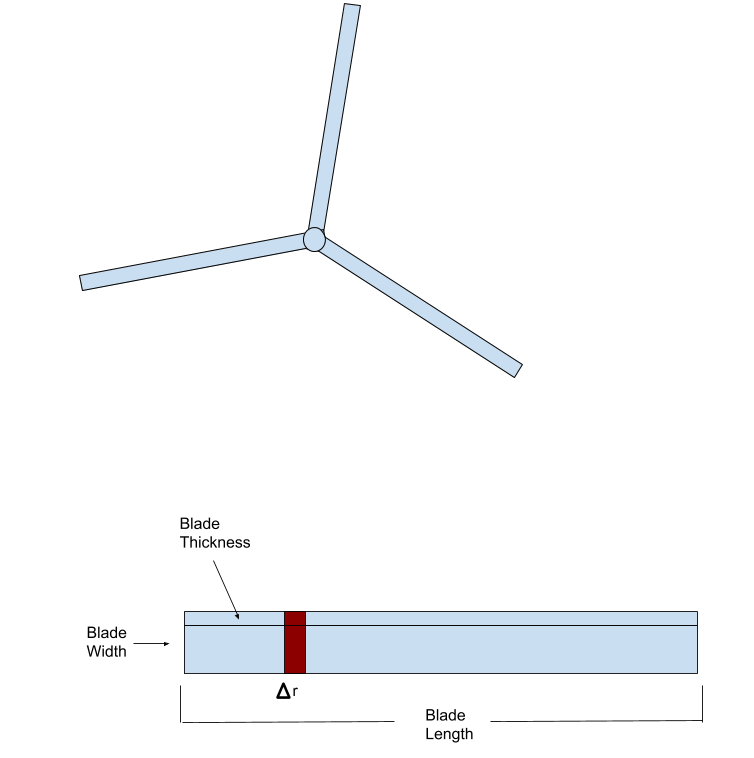
\includegraphics[scale=0.34]{blade}\\
\vspace{0.5\baselineskip} % Whitespace before the editors


{\LARGE Get Mass of Slice \\} % Title
\vspace{0.5\baselineskip} % Whitespace before the editors
\vspace{0.5\baselineskip} % Whitespace before the editors

\textit{Kinetic Energy = $\frac{1}{2}*$(mass)(linear velocity)$^2$}\\

\vspace{0.5\baselineskip} % Whitespace before the editors
\vspace{0.5\baselineskip} % Whitespace before the editors

Our first step is to get the mass of an individual slice. We do this by breaking down the formula for mass into smaller parts that we can directly relate to the helicopter blade. Below is the formula for mass.\\

\vspace{0.5\baselineskip} % Whitespace before the editors
\vspace{0.5\baselineskip} % Whitespace before the editors

\textit{mass = volume $*$ density}\\

\vspace{0.5\baselineskip} % Whitespace before the editors
\vspace{0.5\baselineskip} % Whitespace before the editors

We then relate this formula to the helicopter blade.\\

\vspace{0.5\baselineskip} % Whitespace before the editors
\vspace{0.5\baselineskip} % Whitespace before the editors

\textit{slice mass = slice volume $*$ blade density}\\

\vspace{0.5\baselineskip} % Whitespace before the editors
\vspace{0.5\baselineskip} % Whitespace before the editors

Slice volume can be simplified further\dots below is a formula for volume.

\vspace{0.5\baselineskip} % Whitespace before the editors
\vspace{0.5\baselineskip} % Whitespace before the editors

\textit{volume = area $*$ thickness}\\

\vspace{0.5\baselineskip} % Whitespace before the editors
\vspace{0.5\baselineskip} % Whitespace before the editors

We then relate this formula to the helicopter blade.\\

\vspace{0.5\baselineskip} % Whitespace before the editors
\vspace{0.5\baselineskip} % Whitespace before the editors

\textit{slice volume = slice area $*$ blade thickness}\\

\vspace{0.5\baselineskip} % Whitespace before the editors
\vspace{0.5\baselineskip} % Whitespace before the editors

Slice area can be simplified further\dots below is a formula for area.

\vspace{0.5\baselineskip} % Whitespace before the editors
\vspace{0.5\baselineskip} % Whitespace before the editors

\textit{area = length $*$ width}\\

\vspace{0.5\baselineskip} % Whitespace before the editors
\vspace{0.5\baselineskip} % Whitespace before the editors

We then relate this formula to the helicopter blade.\\

\vspace{0.5\baselineskip} % Whitespace before the editors
\vspace{0.5\baselineskip} % Whitespace before the editors

\textit{slice area = $\Delta$radius $*$ blade width}\\

\vspace{0.5\baselineskip} % Whitespace before the editors
\vspace{0.5\baselineskip} % Whitespace before the editors

We have now simplified the formula for mass and related it directly to the helicopter blade.\\

\vspace{0.5\baselineskip} % Whitespace before the editors
\vspace{0.5\baselineskip} % Whitespace before the editors

\textit{slice mass = blade width $*$ blade thickness $*$ blade density $*$ $\Delta$radius}\\

\vspace{0.5\baselineskip} % Whitespace before the editors
\vspace{0.5\baselineskip} % Whitespace before the editors

{\LARGE Get Linear Velocity of Slice \\} % Title
\vspace{0.5\baselineskip} % Whitespace before the editors
\vspace{0.5\baselineskip} % Whitespace before the editors

Our next step is to get the linear velocity of an individual slice. Again we will break down the formula for linear velocity as it relates to angular velocity.\\

\vspace{0.5\baselineskip} % Whitespace before the editors
\vspace{0.5\baselineskip} % Whitespace before the editors

\textit{linear velocity = angular velocity $*$ radius}\\

\vspace{0.5\baselineskip} % Whitespace before the editors
\vspace{0.5\baselineskip} % Whitespace before the editors

We then relate this to the helicopter blade.\\

\vspace{0.5\baselineskip} % Whitespace before the editors
\vspace{0.5\baselineskip} % Whitespace before the editors

\textit{slice linear velocity = blade angular velocity $*$ radius}\\

\vspace{0.5\baselineskip} % Whitespace before the editors
\vspace{0.5\baselineskip} % Whitespace before the editors

We have now simplified formulas for mass and linear velocity as they relate to the helicopter blade. We can now plug these into our formula for kinetic energy and use an integral to consider each slice.\\

\vspace{0.5\baselineskip} % Whitespace before the editors
\vspace{0.5\baselineskip} % Whitespace before the editors

\textit{kinetic energy = $\frac{1}{2} \int_{0}^{R}$slice mass $*$ slice linear velocity$^2$ dr}\\

\vspace{0.5\baselineskip} % Whitespace before the editors
\vspace{0.5\baselineskip} % Whitespace before the editors

We will now plug our simplifications for slice mass and slice linear velocity into this integral.\\

\vspace{0.5\baselineskip} % Whitespace before the editors
\vspace{0.5\baselineskip} % Whitespace before the editors

\textit{kinetic energy = $\frac{1}{2} \int_{0}^{R}$((blade width $*$ blade thickness) $*$ blade density) $*$ (blade angular velocity $*$ r)$^2$ dr}

\vspace{0.5\baselineskip} % Whitespace before the editors
\vspace{0.5\baselineskip} % Whitespace before the editors

This formula now shows us what characteristics of the helicopter blade we should research to estimate the kinetic energy. We need to find values for blade width, blade thickness, blade density, and blade angular velocity. Below is a table with the values we found.\\

\begin{table}[!h]
\centering
\begin{tabular}{|l|l|l|l|}
\hline
Width    & Thickness & Density      & Angular Velocity ($\omega$) \\ \hline
0.6095 m & 0.0507 m  & 7700 $\frac{kg}{m^3}$  & 52.359 $\frac{rad}{s}$         \\ \hline
(2 ft)   & (2 in)    & (7.7 $\frac{g}{cm^3}$) & (500 rpm)            \\ \hline
\end{tabular}
\end{table}

\vspace{0.5\baselineskip} % Whitespace before the editors
\vspace{0.5\baselineskip} % Whitespace before the editors

We have decided to calculate the kinetic energy for the blade of an Apache helicopter made out of aircraft steel. We first found that the length of the blade is 24 ft. We then convert this to meters.

\vspace{0.5\baselineskip} % Whitespace before the editors
\vspace{0.5\baselineskip} % Whitespace before the editors

$24ft * \frac{1m}{3.28084ft} = 7.315m$\\

\vspace{0.5\baselineskip} % Whitespace before the editors
\vspace{0.5\baselineskip} % Whitespace before the editors

We then found that the width of a blade is typically 2 ft, and again we convert this to meters.\\

\vspace{0.5\baselineskip} % Whitespace before the editors
\vspace{0.5\baselineskip} % Whitespace before the editors

$2ft * \frac{1m}{3.28084ft} = 0.6095m$\\

\vspace{0.5\baselineskip} % Whitespace before the editors
\vspace{0.5\baselineskip} % Whitespace before the editors

We then found that the thickness of a blade is typically 2 in. Once again we convert this to meters.\\

\vspace{0.5\baselineskip} % Whitespace before the editors
\vspace{0.5\baselineskip} % Whitespace before the editors

$2in * \frac{1m}{39.3701in} = 0.0507m$\\

\vspace{0.5\baselineskip} % Whitespace before the editors
\vspace{0.5\baselineskip} % Whitespace before the editors

We also found on wikipedia that the density of aircraft steel is $7.7 \frac{g}{cm^3}$, which we then convert.\\

\vspace{0.5\baselineskip} % Whitespace before the editors
\vspace{0.5\baselineskip} % Whitespace before the editors

$7.7\frac{g}{cm^3}*(\frac{1kg}{1000g})*(\frac{1000000cm^3}{1m^3}) = 7700\frac{kg}{m^3}$\\

\vspace{0.5\baselineskip} % Whitespace before the editors
\vspace{0.5\baselineskip} % Whitespace before the editors

Finally we found that at max speed, an apache helicopter blade is typically rotating at 500 rpms. We need to convert this to $\frac{radians}{second}$.\\

\vspace{0.5\baselineskip} % Whitespace before the editors
\vspace{0.5\baselineskip} % Whitespace before the editors

$(500 \frac{rev}{min})*(\frac{1min}{60s})*(2 \frac{rad}{1rev}) = 52.359 \frac{rad}{s}$\\

\vspace{0.5\baselineskip} % Whitespace before the editors
\vspace{0.5\baselineskip} % Whitespace before the editors


{\LARGE Check Units \\} % Title
\vspace{0.5\baselineskip} % Whitespace before the editors
\vspace{0.5\baselineskip} % Whitespace before the editors

To confirm our previous work we are going to check the units of our formula given these values. Kinetic energy is typically measured in Joules:\\

\vspace{0.5\baselineskip} % Whitespace before the editors
\vspace{0.5\baselineskip} % Whitespace before the editors

$J = \frac{(1kg*m^2)}{(s^2)}$\\

\vspace{0.5\baselineskip} % Whitespace before the editors
\vspace{0.5\baselineskip} % Whitespace before the editors

The units for our formula are:\\

\vspace{0.5\baselineskip} % Whitespace before the editors
\vspace{0.5\baselineskip} % Whitespace before the editors

$m*m*(\frac{kg}{m^3})*(\frac{rad}{s} * m)^2*m$\\

\vspace{0.5\baselineskip} % Whitespace before the editors
\vspace{0.5\baselineskip} % Whitespace before the editors

$kg*\frac{m^2}{s^2}$\\ 

\vspace{0.5\baselineskip} % Whitespace before the editors
\vspace{0.5\baselineskip} % Whitespace before the editors

{\LARGE Estimate Kinetic Energy \\} % Title
\vspace{0.5\baselineskip} % Whitespace before the editors
\vspace{0.5\baselineskip} % Whitespace before the editors

As you can see the units for our formula model the units for Jules. This gives us confidence that the formula we derived for kinetic energy is accurate. Now we can plug assumed values into our formula to start estimating the kinetic energy of the helicopter blade.\\

\vspace{0.5\baselineskip} % Whitespace before the editors
\vspace{0.5\baselineskip} % Whitespace before the editors

\textit{kinetic energy = $\frac{1}{2} \int_{0}^{7.315}((0.6095 *0.0507) *7700) * (52.395 * r)^2 dr$}\\

\vspace{0.5\baselineskip} % Whitespace before the editors
\vspace{0.5\baselineskip} % Whitespace before the editors

\textit{kinetic energy = 42,613,168.254877 Joules}\\

\vspace{0.5\baselineskip} % Whitespace before the editors
\vspace{0.5\baselineskip} % Whitespace before the editors

Our estimation for the kinetic energy of a 24 foot Apache Helicopter Blade made out of aircraft steel is 42,613,168.254877 Joules. This estimate was heavily dependent on assumptions. Specifically the width of the blade had to be estimated based on a picture where the length and thickness were given. Additionally we assumed that this helicopter blade was made out of aircraft steel. This is common, but not always the case. We are again confident in our integral given that the units for Joules can be derived from it. Despite this, we recognize that there is certainly error in our final answer given the assumptions we were forced to make.\\

\vspace{0.5\baselineskip} % Whitespace before the editors
\vspace{0.5\baselineskip} % Whitespace before the editors
---------------------------------------------------------------------------------------------------------
\vspace{0.5\baselineskip} % Whitespace before the editors
\vspace{0.5\baselineskip} % Whitespace before the editors

{\LARGE The Earth \\} % Title
\vspace{0.5\baselineskip} % Whitespace before the editors
\vspace{0.5\baselineskip} % Whitespace before the editors

The next problem asks us to consider the kinetic energy of the Earth as it rotates about its axis. It is again important to use an integral when calculating this value specifically because the Earth is rotating about its axis. This problem is very similar to the record, however we are not dealing with a sphere instead of a cylinder. \\

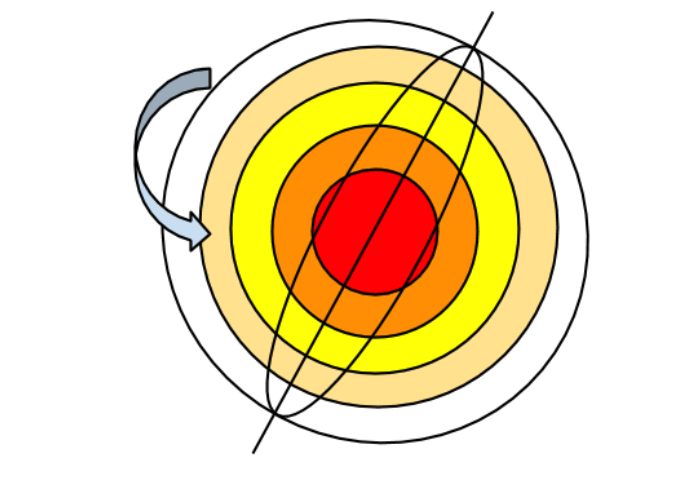
\includegraphics[scale=0.5]{earth2}\\

{\LARGE Get Mass of Slice \\} % Title
\vspace{0.5\baselineskip} % Whitespace before the editors
\vspace{0.5\baselineskip} % Whitespace before the editors

Our first step is to get the mass of an individual slice. We are thinking of our slices similar to the record, however we will consider the circular slice radiating out from the center as a sphere. We start this process by breaking down the formula for mass into smaller parts that we can directly relate to the earth. Below is the formula for mass. \\

\vspace{0.5\baselineskip} % Whitespace before the editors
\vspace{0.5\baselineskip} % Whitespace before the editors

\textit{mass = volume $*$ density}\\

\vspace{0.5\baselineskip} % Whitespace before the editors
\vspace{0.5\baselineskip} % Whitespace before the editors

\textit{We then relate this formula to the earth.}\\

\vspace{0.5\baselineskip} % Whitespace before the editors
\vspace{0.5\baselineskip} % Whitespace before the editors

\textit{slice mass = slice volume $*$ earth density}\\

\vspace{0.5\baselineskip} % Whitespace before the editors
\vspace{0.5\baselineskip} % Whitespace before the editors

Slice volume can be simplified further\dots below is a formula for volume.\\

\vspace{0.5\baselineskip} % Whitespace before the editors
\vspace{0.5\baselineskip} % Whitespace before the editors

\textit{volume = area $*$ thickness}\\

\vspace{0.5\baselineskip} % Whitespace before the editors
\vspace{0.5\baselineskip} % Whitespace before the editors

We then relate this formula to the helicopter blade.\\

\vspace{0.5\baselineskip} % Whitespace before the editors
\vspace{0.5\baselineskip} % Whitespace before the editors

\textit{slice volume = slice area $*$  $\Delta$radius}\\

\vspace{0.5\baselineskip} % Whitespace before the editors
\vspace{0.5\baselineskip} % Whitespace before the editors

Slice area can be simplified further\dots below is a formula for area.\\

\vspace{0.5\baselineskip} % Whitespace before the editors
\vspace{0.5\baselineskip} % Whitespace before the editors

\textit{area = length $*$ width}\\

\vspace{0.5\baselineskip} % Whitespace before the editors
\vspace{0.5\baselineskip} % Whitespace before the editors

We then relate this formula to the helicopter blade.\\

\vspace{0.5\baselineskip} % Whitespace before the editors
\vspace{0.5\baselineskip} % Whitespace before the editors

\textit{slice area = $\pi(\sqrt{(R^2-r^2)})^2$}\\

\vspace{0.5\baselineskip} % Whitespace before the editors
\vspace{0.5\baselineskip} % Whitespace before the editors

We have now simplified the formula for mass and related it directly to the Earth.\\

\vspace{0.5\baselineskip} % Whitespace before the editors
\vspace{0.5\baselineskip} % Whitespace before the editors

\textit{slice mass = $\pi(\sqrt{(R^2-r^2)})^2 * $ earth density $*$ $\Delta$radius}\\

\vspace{0.5\baselineskip} % Whitespace before the editors
\vspace{0.5\baselineskip} % Whitespace before the editors

{\LARGE Get Linear Velocity of Slice \\} % Title
\vspace{0.5\baselineskip} % Whitespace before the editors
\vspace{0.5\baselineskip} % Whitespace before the editors

Our next step is to get the linear velocity of an individual slice. Again we will break down the formula for linear velocity as it relates to angular velocity.\\

\vspace{0.5\baselineskip} % Whitespace before the editors
\vspace{0.5\baselineskip} % Whitespace before the editors

\textit{linear velocity = angular velocity $*$ radius}\\

\vspace{0.5\baselineskip} % Whitespace before the editors
\vspace{0.5\baselineskip} % Whitespace before the editors

We then relate this to the Earth.\\

\vspace{0.5\baselineskip} % Whitespace before the editors
\vspace{0.5\baselineskip} % Whitespace before the editors

\textit{slice linear velocity = earth angular velocity $*$ radius}\\

\vspace{0.5\baselineskip} % Whitespace before the editors
\vspace{0.5\baselineskip} % Whitespace before the editors

We have now simplified formulas for mass and linear velocity as they relate to the earth. We can now plug these into our formula for kinetic energy and use an integral to consider each slice.\\

\vspace{0.5\baselineskip} % Whitespace before the editors
\vspace{0.5\baselineskip} % Whitespace before the editors

\textit{kinetic energy = $\frac{1}{2} \int_{0}^{R}$ slice mass $*$ slice linear velocity$^2$ dr}\\

\vspace{0.5\baselineskip} % Whitespace before the editors
\vspace{0.5\baselineskip} % Whitespace before the editors

We will now plug our simplifications for slice mass and slice linear velocity into this integral.\\

\vspace{0.5\baselineskip} % Whitespace before the editors
\vspace{0.5\baselineskip} % Whitespace before the editors

\textit{kinetic energy = $\frac{1}{2} \int_{0}^{R}((\pi(\sqrt{(R^2-r^2)})^2) *$ earth density) $*$ (earth angular velocity $*$ r)$^2$dr}\\

\vspace{0.5\baselineskip} % Whitespace before the editors

This formula now shows us what characteristics of the Earth we should research to estimate the kinetic energy. We need to find values for Earth radius, Earth density, and Earth angular velocity. Below is a table with the values we found.\\

\begin{table}[!h]
\centering
\begin{tabular}{|l|l|l|l|}
\hline
Layer        & Density                    & Thickness          & Angular Velocity                 \\ \hline
Crust        & 2500 $\frac{kg}{m^3} (2.5 \frac{g}{cm^3})$    & 30000m(30 km)      & 0.0000726755 $\frac{rad}{s}$ (0.000694 rpm) \\ \hline
Upper Mantle & 4000 $\frac{kg}{m^3} (4 \frac{g}{cm^3})$      & 720000m(720 km)    & 0.0000726755 $\frac{rad}{s}$ (0.000694 rpm) \\ \hline
Lower Mantle & 5100 $\frac{kg}{m^3} (5.1 \frac{gm}{cm^3)}$   & 2171000m(2,171 km) & 0.0000726755 $\frac{rad}{s}$ (0.000694 rpm) \\ \hline
Outer Core   & 11200 $\frac{kg}{m^3} (11.2 \frac{gm}{cm^3)}$ & 2259000m(2,259 km) & 0.0000726755 $\frac{rad}{s}$ (0.000694 rpm) \\ \hline
Inner Core   & 12900 $\frac{kg}{m^3} (12.9 \frac{gm}{cm^3)}$ & 1221000m(1,221 km) & 0.0000726755 $\frac{rad}{s}$ (0.000694 rpm) \\ \hline
\end{tabular}
\end{table}

\vspace{0.5\baselineskip} % Whitespace before the editors
\vspace{0.5\baselineskip} % Whitespace before the editors

We found during our research that the earth has five distinct layers, each with a specific thickness and density. Instead of creating a formula to capture this changing density, we are going to calculate each interval separately.\\

\vspace{0.5\baselineskip} % Whitespace before the editors
\vspace{0.5\baselineskip} % Whitespace before the editors

{\LARGE Check Units \\} % Title
\vspace{0.5\baselineskip} % Whitespace before the editors
\vspace{0.5\baselineskip} % Whitespace before the editors

To confirm our previous work we are going to check the units of our formula given these values. Kinetic energy is typically measured in Joules:\\

\vspace{0.5\baselineskip} % Whitespace before the editors
\vspace{0.5\baselineskip} % Whitespace before the editors

$J=\frac{1kg * m^2}{s^2}$\\

\vspace{0.5\baselineskip} % Whitespace before the editors
\vspace{0.5\baselineskip} % Whitespace before the editors

The units for our formula are:\\

\vspace{0.5\baselineskip} % Whitespace before the editors
\vspace{0.5\baselineskip} % Whitespace before the editors

$m^2 * (\frac{kg}{m^3})*(\frac{rad}{s} * m)^2*m$\\

\vspace{0.5\baselineskip} % Whitespace before the editors
\vspace{0.5\baselineskip} % Whitespace before the editors

$kg * \frac{m^2}{s^2}$\\ 

\vspace{0.5\baselineskip} % Whitespace before the editors
\vspace{0.5\baselineskip} % Whitespace before the editors

{\LARGE Estimate Kinetic Energy \\} % Title
\vspace{0.5\baselineskip} % Whitespace before the editors
\vspace{0.5\baselineskip} % Whitespace before the editors

Finally we will estimate the kinetic energy for each layer of the earth.\\

\vspace{0.5\baselineskip} % Whitespace before the editors
\vspace{0.5\baselineskip} % Whitespace before the editors
%------------------------------------------------------------------------------------------------------------
\textbf{\textit{inner core kinetic energy = }}\\

\vspace{0.5\baselineskip} % Whitespace before the editors
\vspace{0.5\baselineskip} % Whitespace before the editors

$\frac{1}{2} \int_{0}^{1221000} ((\pi(\sqrt{1221000^2-r^2})^2) * 12900) * (0.0000726755 * r)^2 dr$\\

\vspace{0.5\baselineskip} % Whitespace before the editors
\vspace{0.5\baselineskip} % Whitespace before the editors

$3.872600528326376*10^{25} Joules$

\vspace{0.5\baselineskip} % Whitespace before the editors
\vspace{0.5\baselineskip} % Whitespace before the editors
%------------------------------------------------------------------------------------------------------------
\textbf{\textit{outer core kinetic energy = }}\\

\vspace{0.5\baselineskip} % Whitespace before the editors
\vspace{0.5\baselineskip} % Whitespace before the editors

$\frac{1}{2} \int_{1221000}^{3840000} ((\pi(\sqrt{3480000^2-r^2})^2) * 11200) * (0.0000726755 * r)^2 dr$\\

\vspace{0.5\baselineskip} % Whitespace before the editors
\vspace{0.5\baselineskip} % Whitespace before the editors

$5.691001160848006*10^{27} Joules$

\vspace{0.5\baselineskip} % Whitespace before the editors
\vspace{0.5\baselineskip} % Whitespace before the editors
%------------------------------------------------------------------------------------------------------------
\textbf{\textit{lower mantle kinetic energy = }}\\

\vspace{0.5\baselineskip} % Whitespace before the editors
\vspace{0.5\baselineskip} % Whitespace before the editors

$\frac{1}{2} \int_{3480000}^{5651000} ((\pi(\sqrt{5651000^2-r^2})^2) * 5100) * (0.0000726755 * r)^2 dr$\\

\vspace{0.5\baselineskip} % Whitespace before the editors
\vspace{0.5\baselineskip} % Whitespace before the editors

$1.784855287866927*10^{28} Joules$

\vspace{0.5\baselineskip} % Whitespace before the editors
\vspace{0.5\baselineskip} % Whitespace before the editors
%------------------------------------------------------------------------------------------------------------
\textbf{\textit{upper mantle kinetic energy = }}\\

\vspace{0.5\baselineskip} % Whitespace before the editors
\vspace{0.5\baselineskip} % Whitespace before the editors

$\frac{1}{2} \int_{5651000}^{6371000} ((\pi(\sqrt{6371000^2-r^2})^2) * 4000) * (0.0000726755 * r)^2 dr$\\

\vspace{0.5\baselineskip} % Whitespace before the editors
\vspace{0.5\baselineskip} % Whitespace before the editors

$3.666394873547232*10^{27} Joules$

\vspace{0.5\baselineskip} % Whitespace before the editors
\vspace{0.5\baselineskip} % Whitespace before the editors
%------------------------------------------------------------------------------------------------------------
\textbf{\textit{crust kinetic energy = }}\\

\vspace{0.5\baselineskip} % Whitespace before the editors
\vspace{0.5\baselineskip} % Whitespace before the editors

$\frac{1}{2} \int_{6371000}^{6401000} ((\pi(\sqrt{6401000^2-r^2})^2) * 2500) * (0.0000726755 * r)^2 dr$\\

\vspace{0.5\baselineskip} % Whitespace before the editors
\vspace{0.5\baselineskip} % Whitespace before the editors

$4.857645575976313*10^{24} Joules$

\vspace{0.5\baselineskip} % Whitespace before the editors
\vspace{0.5\baselineskip} % Whitespace before the editors
%------------------------------------------------------------------------------------------------------------
Adding these results together we get 2.7249532563923748073$*10^{28}$, or twenty-seven octillion, two hundred forty-nine septillion, five hundred thirty-two sextillion, five hundred sixty-three quintillion, nine hundred twenty-three quadrillion, seven hundred forty-eight trillion, seventy-three billion Joules.\\

\vspace{0.5\baselineskip} % Whitespace before the editors
\vspace{0.5\baselineskip} % Whitespace before the editors

We our confident that our math is accurate, however, we made many assumptions in this calculation. One assumption is that the earth is a perfect sphere, without mountains or valleys. We are hoping that the sum of the mass of these irregularities in the Earth's surface is insignificant when considering the mass of the earth as a whole. Additionally we made assumptions about the thickness and density of the different layers within the earth. We also assumed that these layers were uniform thicknesses.\\

\vspace{0.5\baselineskip} % Whitespace before the editors
\vspace{0.5\baselineskip} % Whitespace before the editors
---------------------------------------------------------------------------------------------------------
\vspace{0.5\baselineskip} % Whitespace before the editors
\vspace{0.5\baselineskip} % Whitespace before the editors

{\LARGE Summation \\} % Title
\vspace{0.5\baselineskip} % Whitespace before the editors
\vspace{0.5\baselineskip} % Whitespace before the editors

In summation, we were able to use our knowledge of integrals to estimate the kinetic energy of various objects rotating about an axis. We were able to account for changing object density when calculating mass, and unit conversions to make our results meaningful. We were able to find our estimates using assumptions such as thinking of objects as more basic shapes and considering them as slices. It was rewarding to watch our understanding of each scenario and the math involved improve throughout the process of completing this report. \\

\vspace{0.5\baselineskip} % Whitespace before the editors
\vspace{0.5\baselineskip} % Whitespace before the editors
---------------------------------------------------------------------------------------------------------
\vspace{0.5\baselineskip} % Whitespace before the editors
\vspace{0.5\baselineskip} % Whitespace before the editors

{\LARGE References \\} % Title
\vspace{0.5\baselineskip} % Whitespace before the editors
\vspace{0.5\baselineskip} % Whitespace before the editors

\textbf{The Record}\\
(1) \url{https://www.vinylengine.com/turntable_forum/viewtopic.php?f=41&t=93648}\\
(2) \url{https://en.wikipedia.org/wiki/Phonograph_record}\\
(3) \url{https://en.wikipedia.org/wiki/LP_record}\\
(4) \url{https://en.wikipedia.org/wiki/Polyvinyl_chloride}\\

\vspace{0.5\baselineskip} % Whitespace before the editors
\vspace{0.5\baselineskip} % Whitespace before the editors

\textbf{The Helicopter Blade}\\
(5) \url{http://www.inetres.com/gp/military/ar/rotor/AH-64.html}\\
(6) \url{https://www.google.com/search?source=hp&ei=aViQXOu-CoPr_Qbq3ZE4&q=steel+density}\\

\vspace{0.5\baselineskip} % Whitespace before the editors
\vspace{0.5\baselineskip} % Whitespace before the editors

\textbf{The Earth}\\
(7) \url{http://hyperphysics.phy-astr.gsu.edu/hbase/Geophys/earthstruct.html}\\
(8) \url{http://www.engineering.com/Ask@/qactid/1/qaqid/3431.aspx}\\
\end{document}
